\documentclass[10pt,twocolumn]{memoir}

% Left and right margins
\setlrmarginsandblock{0.35in}{0.35in}{*}
% Top and bottom margins
\setulmarginsandblock{1in}{0.8in}{*}
% Apply the layout
\checkandfixthelayout
% Space between the two columns
\setlength{\columnsep}{0.2in}
% Space between paragrahps
% \setlength{\parskip}{0.1em}
% Indentation before paragraphs
% \setlength{\parindent}{1em}

\usepackage{microtype}
\usepackage{mathpazo}
\usepackage{amsmath}
\usepackage{tikz}
\usetikzlibrary{arrows.meta,patterns.meta,calc}

\begin{document}

\chapter{Introduction}
\label{ch:introduction}

\section{Dynamic Meteorology}

Weather phenomena occur in the troposphere, the lowest part of the atmosphere in contact with Earth's surface. The troposphere extends on average to about $10\,\mathrm{km}$ above the surface, with the tropopause marking its upper boundary.

The laws of atmospheric motion must satisfy the \textit{principle of dimensional homogeneity}, meaning that all terms in an equation must have consistent physical dimensions. Four dimensionally independent physical properties are sufficient to describe all quantities used in atmospheric dynamics: length, mass, time, and thermodynamic temperature. In the International System of Units (SI), these properties are measured using the base units shown in Table~\ref{tab:c1_base_units}. All other physical quantities are expressed in derived units formed from products or ratios of these base units. A number of important derived units have special names and symbols, as indicated in Table~\ref{tab:c1_derived_units}.

\begin{table}[h]
\centering
\caption{SI Basis Units}
\begin{tabular}{lll}
\hline
Property & Name & Symbol \\
\hline
Length      & Meter    & $\mathrm{m}$  \\
Mass        & Kilogram & $\mathrm{kg}$ \\
Time        & Second   & $\mathrm{s}$  \\
Temperature & Kelvin   & $\mathrm{K}$  \\
\hline
\end{tabular}
\label{tab:c1_base_units}
\end{table}

\begin{table}[h]
\centering
\caption{SI Derived Units with Special Names}
\begin{tabular}{lll}
\hline
Property & Name & Symbol \\
\hline
Frequency & Hertz  & $\mathrm{s^{-1}}$ \\
Force     & Newton & $\mathrm{N}\;(\mathrm{kg\,m\,s^{-2}})$ \\
Pressure  & Pascal & $\mathrm{Pa}\;(\mathrm{N\,m^{-2}})$ \\
Energy    & Joule  & $\mathrm{J}\;(\mathrm{N\,m})$ \\
Power     & Watt   & $\mathrm{W}\;(\mathrm{J\,s^{-1}})$ \\
\hline
\end{tabular}
\label{tab:c1_derived_units}
\end{table}

Dynamic meteorology applies the conservation laws of momentum, mass, and energy to the atmosphere. This treatment relies on the \textit{continuum approximation}, in which the discrete molecular structure of air is replaced by continuous field variables such as pressure, density, and temperature that vary smoothly in space and time. A ``point'' in this continuum, often called an \textit{air parcel} or \textit{air particle}, represents a volume that is very small relative to the atmosphere but still contains many molecules. This approximation allows the conservation laws to be applied to small atmospheric volume elements to derive the governing equations of atmospheric motion.

\section{Conservation of Momentum}

Atmospheric forces can be classified as \textit{body forces} and \textit{surface forces}. Body forces act on the mass of an air parcel and have magnitudes proportional to the mass of the parcel (e.g. gravity), and surface forces act across the parcel boundary and have magnitudes independent of the mass of the parcel (e.g. pressure force). The primary \textit{fundamental forces} controlling atmospheric motion are the pressure gradient force, gravitational force, and frictional force; these determine acceleration measured in a coordinate system fixed in space. When motion is described in a coordinate system rotating with Earth, the centrifugal and Coriolis forces must also be included as \textit{apparent forces}.

\subsection{Pressure Gradient Force}

Pressure is defined as the force per unit area acting normal to a surface. In a gas such as the atmosphere, random molecular motion causes pressure at a point to act equally in all directions, so its magnitude is independent of the orientation of the surface. If pressure differs across a fluid element, the resulting imbalance produces a net force directed toward lower pressure; this is the \textit{pressure gradient force}.

\begin{figure}[h]
\centering
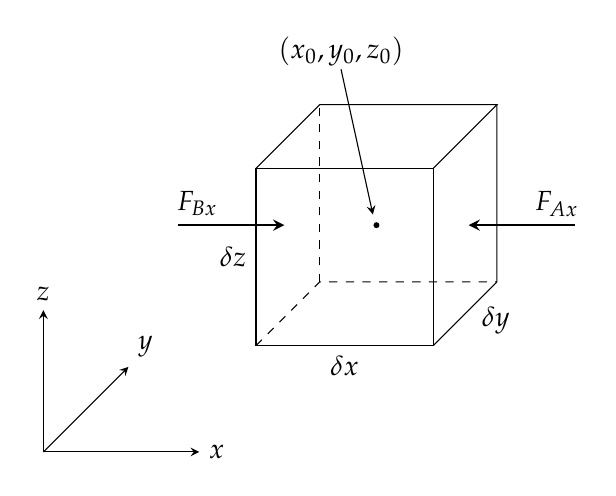
\begin{tikzpicture}[scale=0.9,>=stealth]

% Axes
\draw[->] (-3.0,-1.5) -- (-0.8,-1.5) node[right] {$x$};
\draw[->] (-3.0,-1.5) -- (-3.0,0.5) node[above] {$z$};
\draw[->] (-3.0,-1.5) -- (-1.8,-0.3) node[above right] {$y$};

% Cube: front face
\coordinate (A) at (0,0);
\coordinate (B) at (2.5,0);
\coordinate (C) at (2.5,2.5);
\coordinate (D) at (0,2.5);

% Back face
\coordinate (E) at (0.9,0.9);
\coordinate (F) at (3.4,0.9);
\coordinate (G) at (3.4,3.4);
\coordinate (H) at (0.9,3.4);

% Visible edges
\draw (A) -- (B) -- (C) -- (D) -- cycle;
\draw (D) -- (H) -- (G) -- (C);
\draw (B) -- (F) -- (G);

% Hidden edges
\draw[dashed] (A) -- (E) -- (F);
\draw[dashed] (E) -- (H);

% Center
\fill (1.7,1.7) circle (1.2pt);
\draw[->] (1.2,3.9) -- (1.65,1.85);
\node at (1.2,4.15) {$(x_0,y_0,z_0)$};

% Pressure forces
\draw[->,thick] (4.5,1.7) -- (3.0,1.7);
\node[right] at (3.8,2.0) {$F_{Ax}$};

\draw[->,thick] (-1.1,1.7) -- (0.4,1.7);
\node[left] at (-0.4,2.0) {$F_{Bx}$};

% Dimensions
\node[below] at (1.25,0) {$\delta x$};
\node[right] at (3.05,0.35) {$\delta y$};
\node[left] at (0,1.25) {$\delta z$};

\end{tikzpicture}
\caption{The $x$ component of the pressure gradient force acting on a cubic fluid element.}
\label{fig:c1_pressure_gradient_force}
\end{figure}

Consider an infinitesimal air parcel with volume

\begin{equation}
    \delta V = \delta x \delta y \delta z,
\end{equation}

centered at $(x_0,y_0,z_0)$, where the pressure at the center is $p_0$. Using a Taylor expansion, the pressures on the two faces normal to the $x$ direction are approximately

\begin{equation}
    p_A = p_0 + \frac{\partial p}{\partial x}\frac{\delta x}{2} + O(\delta x^2),
\end{equation}

and

\begin{equation}
    p_B = p_0 - \frac{\partial p}{\partial x}\frac{\delta x}{2} + O(\delta x^2),
\end{equation}

Since pressure acts inward on each face, the force on face $A$ is directed opposite to the positive $x$ direction and therefore carries a negative sign, whereas the force on face $B$ is directed along the positive $x$ direction. Thus,

\begin{equation}
    F_{Ax} = -\left(p_0+\frac{\partial p}{\partial x}\frac{\delta x}{2}
    \right)\delta y \delta z,
\end{equation}

and

\begin{equation}
    F_{Bx} = \left(p_0-\frac{\partial p}{\partial x}\frac{\delta x}{2}
    \right)\delta y \delta z.
\end{equation}

Adding the two contributions gives the net pressure force in the $x$ direction,

\begin{equation}
    F_x = F_{Ax}+F_{Bx} = -\frac{\partial p}{\partial x}\delta x \delta y \delta z.
\end{equation}

The mass of the parcel is

\begin{equation}
    m = \rho\delta x \delta y\delta z,
\end{equation}

so the pressure gradient force per unit mass in the $x$ direction is

\begin{equation}
    \frac{F_x}{m} = -\frac{1}{\rho}\frac{\partial p}{\partial x}.
\end{equation}

Applying the same argument in the $y$ and $z$ directions gives

\begin{equation}
    \frac{F_y}{m} = -\frac{1}{\rho}\frac{\partial p}{\partial y},
    \qquad
    \frac{F_z}{m} = -\frac{1}{\rho}\frac{\partial p}{\partial z}.
\end{equation}

Therefore, the total pressure gradient force per unit mass can be written in vector form as

\begin{equation}
    \frac{\mathbf{F}}{m} = -\frac{1}{\rho}\nabla p = -\frac{1}{\rho}\left<\frac{\partial p}{\partial x};\frac{\partial p}{\partial y};\frac{\partial p}{\partial z}\right>,
\end{equation}

where $\nabla$ denotes the gradient operator,

\begin{equation}
    \nabla = \left<\frac{\partial}{\partial x}; \frac{\partial}{\partial y}; \frac{\partial}{\partial z}\right>
\end{equation}

Since $\nabla p$ points toward increasing pressure, the negative sign implies that the pressure gradient force points from high pressure toward low pressure. Its magnitude depends on the spatial gradient of the pressure field, rather than on the pressure itself.

\subsection{Viscous Force}

\textit{Viscosity} represents the internal friction of a fluid and arises when the fluid velocity varies in space. Because molecules move randomly between neighboring air parcels, they carry momentum across parcel boundaries, producing a net transfer from faster-moving parcels to slower-moving parcels. This momentum exchange gives rise to a viscous force acting along the face of an air parcel. The corresponding \textit{shear stress} is the viscous force per unit area,

\begin{equation}
    \tau = \frac{F}{A}.
\end{equation}

For a Newtonian fluid such as air, the shear stress is proportional to the velocity gradient. For example, if the $x$ component of velocity $u$ varies with height $z$, the vertical shear produces

\begin{equation}
    \tau_{zx} = \mu \frac{\partial u}{\partial z},
\end{equation}

where $\mu$ is the dynamic viscosity coefficient. Here, $\partial u/\partial z$ measures the rate at which the horizontal velocity component $u$ changes with height. Since $u$ varies with $z$, the shear stress $\tau_{zx}$ is also a function of $z$.

To determine the resulting viscous force, consider an air parcel of thickness $\delta z$ and horizontal area $A=\delta x \delta y$, with mass

\begin{equation}
    m = \rho A\,\delta z.
\end{equation}

The shear stresses on the upper and lower faces act in opposite directions because each neighboring layer tends to drag the parcel toward its own velocity. For a velocity that increases with height, the faster-moving air above pulls the upper face forward, and the slower-moving air below pulls the lower face backward. Thus, the net viscous force in the $x$ direction due to vertical shear is

\begin{equation}
\begin{aligned}
    F_{\mathrm{net}}
    = F_\mathrm{upper} - F_\mathrm{lower} &= A\left[\tau_{zx}(z+\delta z) - \tau_{zx}(z)\right] \\
    &= A\frac{\partial \tau_{zx}}{\partial z}\delta z + O(\delta z^2),
\end{aligned}
\end{equation}

where the last step follows from a Taylor expansion. Dividing by the parcel mass gives the viscous force per unit mass,

\begin{equation}
    \frac{F_{\mathrm{net}}}{m} = \frac{1}{\rho}\frac{\partial \tau_{zx}}{\partial z} = \frac{1}{\rho}\frac{\partial}{\partial z}\left(\mu\frac{\partial u}{\partial z}\right).
\end{equation}

If $\mu$ and $\rho$ are approximately constant, this becomes

\begin{equation}
    \frac{F_{\mathrm{net}}}{m} = \nu\frac{\partial^2 u}{\partial z^2},
\end{equation}

where

\begin{equation}
    \nu = \frac{\mu}{\rho}
\end{equation}

is the \textit{kinematic viscosity coefficient}. Under standard atmospheric conditions at sea level, $\nu \simeq 1.46\times10^{-5}\,\mathrm{m^2\,s^{-1}}$.

The previous expression considers only the diffusion of the $x$ component of momentum, $u$, caused by its variation in the vertical direction $z$ (it is called \textit{diffusion} because it tends to smooth out spatial differences in the velocity field). In general, each velocity component $(u,v,w)$ may vary in all three spatial directions $(x,y,z)$, so momentum can be transferred across surfaces normal to any coordinate direction. Accordingly, the shear stress varies with position, $\tau=\tau(x,y,z)$, and the resulting viscous force includes contributions from all three directions. The frictional force components per unit mass are therefore

\begin{equation}
\begin{aligned}
    F_{rx}
    &= \nu\left(\frac{\partial^2 u}{\partial x^2} + \frac{\partial^2 u}{\partial y^2} + \frac{\partial^2 u}{\partial z^2}\right) = \nu\nabla^2u, \\
    F_{ry}
    &= \nu\left(\frac{\partial^2 v}{\partial x^2} + \frac{\partial^2 v}{\partial y^2} + \frac{\partial^2 v}{\partial z^2}\right) = \nu\nabla^2v, \\
    F_{rz}
    &= \nu\left(\frac{\partial^2 w}{\partial x^2} + \frac{\partial^2 w}{\partial y^2} + \frac{\partial^2 w}{\partial z^2}\right) = \nu\nabla^2w.
\end{aligned}
\end{equation}

where $\nabla^2$ is the Laplacian operator

\begin{equation}
    \nabla^2 u = \nabla\cdot\nabla u = \frac{\partial^2u}{\partial x^2} + \frac{\partial^2u}{\partial y^2} + \frac{\partial^2u}{\partial z^2}.
\end{equation}

The viscous force therefore represents \textit{diffusion of momentum}. At a local maximum of $u$, the gradient vectors converge toward the maximum, giving $\nabla^2u<0$ and causing momentum to be removed from that region. At a local minimum, the gradient vectors diverge and $\nabla^2u>0$, causing momentum to be added. Momentum therefore diffuses downgradient, from regions of larger values toward regions of smaller values.

Below approximately $100\,\mathrm{km}$ in the atmosphere, molecular viscosity is sufficiently small that it is usually negligible, except within a thin layer of a few centimeters near Earth's surface where vertical shear can be very large. Thus, most of the atmosphere can be treated as effectively inviscid with respect to molecular viscosity. Away from the immediate surface, momentum transport is instead dominated by turbulent eddy motions.

\subsection{Gravitational Force}

The sole body force acting on atmospheric air parcels is gravity. According to Newton's law of universal gravitation, if two masses $M$ and $m$ separated by a distance $r=|\mathbf{r}|$ with $\mathbf{r}$ directed from $M$ toward $m$, then the gravitational force exerted by $M$ on $m$ is

\begin{equation}
    \mathbf{F}_g = -\frac{GMm}{r^2}\frac{\mathbf{r}}{r}
\end{equation}

where $G = 6.67430\times10^{-11}\,\mathrm{m^3\,kg^{-1}\,s^{-2}}$ is the universal gravitational constant. The negative sign indicates that the gravitational force is directed opposite to $\mathbf{r}$, toward the attracting mass $M$. For bodies of finite extent, $r$ is interpreted as the distance between their centers of mass.

Taking $M$ to be the mass of Earth and $m$ to be the mass of an atmospheric air parcel, the gravitational force per unit mass is

\begin{equation}
    \frac{\mathbf{F}_g}{m} = \mathbf{g}^* = -\frac{GM}{r^2}\frac{\mathbf{r}}{r}
\end{equation}

where $\mathbf{g}^*$ is the \textit{gravitational acceleration}. In dynamic meteorology, height above mean sea level is commonly used as the vertical coordinate. If $a$ is the mean radius of Earth and $z$ is the height above mean sea level, then

\begin{equation}
    r = a+z.
\end{equation}

Therefore,

\begin{equation}
    \mathbf{g}^* = -\frac{GM}{(a+z)^2}\frac{\mathbf{r}}{r}.
\end{equation}

At mean sea level, $z=0$, so

\begin{equation}
    \mathbf{g}_0^* = -\frac{GM}{a^2}\frac{\mathbf{r}}{r}.
\end{equation}

The gravitational acceleration can now be rewritten as

\begin{equation}
    \mathbf{g}^* = \mathbf{g}_0^*\frac{a^2}{(a+z)^2} = \frac{\mathbf{g}_0^*}{(1+z/a)^2}
\end{equation}

For meteorological applications, $z\ll a$, so the variation of gravitational acceleration with height is very small and, with negligible error, it can be treated as approximately constant,

\begin{equation}
    \mathbf{g}^* \simeq \mathbf{g}_0^*.
\end{equation}

\section{Nonenertial Reference Frame and Apparent Forces}

An \textit{inertial reference frame} is a coordinate system fixed in space. In this frame, Newton's first law applies directly: an object remains at rest or moves with constant velocity unless acted upon by a net force. Motion with these characteristics is called \textit{inertial motion}.

A geocentric reference frame fixed to the rotating Earth is a \textit{noninertial reference frame} because it accelerates relative to a frame fixed in space. An object that appears stationary or in uniform motion in this rotating frame may therefore still be accelerating relative to space. Newton's laws can still be applied in this rotating frame by accounting for the acceleration of the coordinate system through \textit{apparent forces}. For uniform rotation, the two principal apparent forces are the \textit{centrifugal force} and the \textit{Coriolis force}.

\subsection{Centripetal Acceleration and Centrifugal Force}

Consider a ball of mass $m$ attached to a string and rotating in a circle of radius $r$ with constant angular velocity $\omega$. In an inertial reference frame, the speed $|\mathbf{V}|$ is constant, but the direction of $\mathbf{V}$ continuously changes. For a sufficiently small angular displacement $\delta\theta$, the arc can be approximated by the chord, so

\begin{equation}
    |\delta\mathbf{V}| = |\mathbf{V}|\,\delta\theta.
\end{equation}


\begin{figure}[t]
\centering
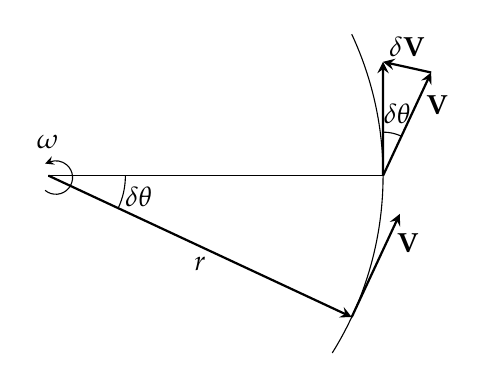
\begin{tikzpicture}[scale=0.85, >=stealth]

% Center of rotation
\coordinate (O) at (0,0);

% Two positions with larger angular separation
\coordinate (P1) at (5,0);
\coordinate (P0) at ({5*cos(-25)},{5*sin(-25)});

% Rotation symbol
\draw (-0.05,-0.22) arc[start angle=-130,end angle=110,radius=0.25];
\draw[->] (0.03,0.21) -- (-0.05,0.18);
\node[left] at (0.3,0.5) {$\omega$};

% Circular trajectory
\draw (O) ++(-32:5) arc[start angle=-32,end angle=25,radius=5];

% Radius vectors
\draw (O) -- (P1);
\draw[->,thick] (O) -- (P0) node[midway,below] {$r$};

% Larger angle at center
\draw (1.15,0) arc[start angle=0,end angle=-25,radius=1.15];
\node at (1.35,-0.32) {$\delta\theta$};

% Velocity at lower position
\draw[->,thick] (P0) -- ++(65:1.7) node[pos=0.72,right] {$\mathbf{V}$};

% Velocity at upper position
\coordinate (Vbase) at (P1);
\coordinate (Vtip) at ($(Vbase)+(65:1.7)$);
\draw[->,thick] (Vbase) -- (Vtip)node[pos=0.68,right] {$\mathbf{V}$};

% Second velocity vector
\coordinate (Vnewtip) at ($(Vbase)+(90:1.7)$);
\draw[->,thick] (Vbase) -- (Vnewtip);

% Change in velocity
\draw[->,thick] (Vtip) -- (Vnewtip) node[midway,above] {$\delta\mathbf{V}$};

% Larger angle between velocity vectors
\draw ($(Vbase)+(65:0.65)$) arc[start angle=65,end angle=90,radius=0.65];
\node at ($(Vbase)+(77:0.95)$) {$\delta\theta$};

\end{tikzpicture}

\caption{Centripetal acceleration results from the change in direction of the velocity vector.}
\label{fig:c1_centripetal_acceleration}
\end{figure}

Hence,

\begin{equation}
    \frac{|\delta\mathbf{V}|}{\delta t} = |\mathbf{V}|\frac{\delta\theta}{\delta t}.
\end{equation}

As $\delta t\rightarrow 0$, the direction of $\delta\mathbf{V}$ approaches the inward radial direction,
$-\mathbf{r}/r$. Therefore,

\begin{equation}
    \frac{D\mathbf{V}}{Dt} = \lim_{\delta t\rightarrow 0}\frac{\delta\mathbf{V}}{\delta t} = |\mathbf{V}|\frac{D\theta}{Dt}\left(-\frac{\mathbf{r}}{r}\right).
\end{equation}

Since $|\mathbf{V}|=\omega r$ and $D\theta/Dt=\omega$,

\begin{equation}
    \frac{D\mathbf{V}}{Dt} = -\omega^2\mathbf{r}.
\end{equation}

This inward acceleration is the \textit{centripetal acceleration}, with magnitude $\omega^2r$, and is produced by the tension in the string.

In a reference frame rotating with the ball, the ball appears stationary even though the string still exerts an inward force. To apply Newton's second law in the rotating frame, the apparent \textit{centrifugal force} must be introduced to balance the centripetal force. It is equal in magnitude and opposite in direction to the centripetal force, and appears only in the noninertial (rotating) frame.

\subsection{Gravity Revisited}

We first choose a Cartesian coordinate system centered at Earth’s center, with the $z$ axis aligned with the rotation axis and the $x$ and $y$ axes lying in the equatorial plane.

In an inertial reference frame, an object fixed to Earth's surface is not generally at rest as Earth rotates. Except at the poles, the object moves in a circle about Earth's rotation axis and therefore requires the centripetal acceleration

\begin{equation}
    \mathbf{a}_c=-\Omega^2\mathbf{R},
\end{equation}

where $\mathbf{R}=x\mathbf{i}+y\mathbf{j}$ is the position vector measured outward and perpendicular to the rotation axis, and $\Omega=7.292\times10^{-5}\,\mathrm{rad\,s^{-1}}$ is Earth's angular speed. Except at the equator and poles, $\mathbf{a}_c$ has both a radial component and a poleward component tangent to the local level surface, as illustrated in Fig.~\ref{fig:c1_radial_horizontal}. A poleward horizontal force is therefore required to produce this component of the centripetal acceleration.

\begin{figure}[t]
\centering
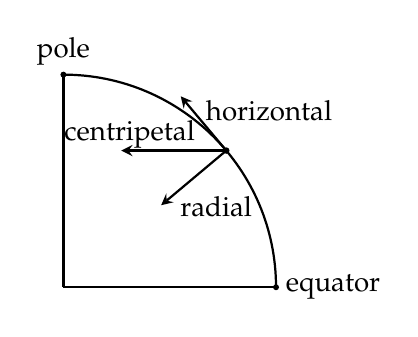
\begin{tikzpicture}[scale=0.9, >=stealth]

% Earth cross-section
\coordinate (C) at (0,0);
\def\R{3}

% Sector representing part of Earth
\draw[thick] (C) -- (0:\R);
\draw[thick] (C) -- (90:\R);
\draw[thick] (0:\R) arc[start angle=0,end angle=90,radius=\R];

% Point on Earth's surface
\coordinate (P) at (40:\R);
\fill (P) circle (1.3pt);

% Radial direction toward Earth's center
\draw[->,thick] (P) -- ++(220:1.2) node[pos=0.5,below right,xshift=-3mm,yshift=-1mm] {radial};

% Local horizontal direction, tangent to Earth's surface
\draw[->,thick] (P) -- ++(130:1.0) node[pos=0.5,above right,xshift=-1mm,yshift=-1mm] {horizontal};

% Centripetal direction, toward axis of rotation
\draw[->,thick] (P) -- ++(180:1.483) node[pos=0.92,above,yshift=-1mm] {centripetal};

% Pole
\fill (90:\R) circle (1.2pt);
\node[above] at (90:\R) {pole};

% Equator
\fill (0:\R) circle (1.2pt);
\node[right] at (0:\R) {equator};

\end{tikzpicture}

\caption{Radial and horizontal components of the centripetal accerleration.}
\label{fig:c1_radial_horizontal}
\end{figure}

Because the centripetal acceleration has a poleward horizontal component regardless of Earth's shape, a corresponding poleward force is required to sustain this component of the centripetal acceleration. If Earth were a homogeneous sphere, the true gravitational acceleration $\mathbf{g}^*$ would point exactly toward Earth's center and could not provide this horizontal force. In reality, Earth is approximately an oblate spheroid, with an equatorial radius about $21\,\mathrm{km}$ larger than its polar radius. The resulting non-uniform mass distribution causes $\mathbf{g}^*$ to deviate slightly from the radial direction (see Fig.~\ref{fig:c1_nonuniform_mass_distribution}), giving it a poleward horizontal component that just sufficiently supplies the required centripetal force.

\begin{figure}[t]
\centering
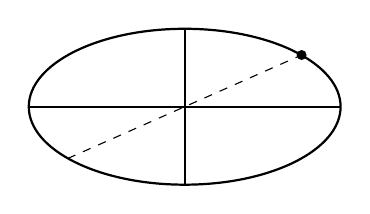
\begin{tikzpicture}[scale=0.9]

% Oblate ellipse
\draw[thick] (0,0) ellipse (2.2 and 1.1);

% Horizontal axis
\draw[thick] (-2.2,0) -- (2.2,0);

% Vertical axis
\draw[thick] (0,-1.1) -- (0,1.1);

% Slanted radius
\draw[dashed] (-1.65,-0.73) -- (1.65,0.73);

% Point on surface
\fill (1.65,0.73) circle (2pt);

\end{tikzpicture}

\caption{Although the dashed line divides the oblate Earth into two equal parts, the mass in the lower part is distributed closer to the surface object. Its gravitational attraction is therefore stronger, causing the true gravitational acceleration $\mathbf{g}^*$ to deviate slightly toward the equator.}

\label{fig:c1_nonuniform_mass_distribution}
\end{figure}

In the rotating frame fixed to Earth (a noninertial reference frame), an object fixed to Earth's surface has no centripetal acceleration relative to the frame. Instead, the inertial-frame centripetal acceleration is replaced by the apparent centrifugal acceleration $\Omega^2\mathbf{R}$, directed outward from the rotation axis. It is therefore convenient to combine the centrifugal acceleration $\Omega^2\mathbf{R}$, and the true gravitational acceleration $\mathbf{g}^*$, to define the effective gravity $\mathbf{g}$ such that,

\begin{equation}
    \mathbf{g} = \mathbf{g}^* + \Omega^2\mathbf{R} = -g\mathbf{k},
\end{equation}

where $g=|\mathbf{g}|$, referred to as \textit{apparent gravity}, and $\mathbf{k}$ is the outward unit vector along the local vertical. The centrifugal contribution partially offsets $\mathbf{g}^*$, so the magnitude of effective gravity is slightly smaller than that of the true gravitational acceleration. As shown in Fig.~\ref{fig:c1_gravity_revisited}, $\mathbf{g}$ defines the local vertical and is perpendicular to Earth's level surface.

\begin{figure}[t]
\centering
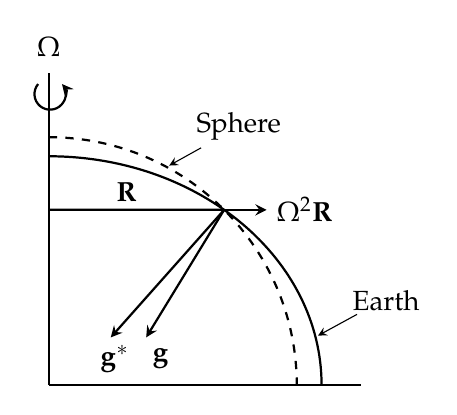
\begin{tikzpicture}[scale=0.9, >=stealth]

% Rotation axis
\draw[thick] (0,0) -- (0,4.4);
\draw[->,thick] (-0.15,4.25) arc[start angle=140,end angle=400,radius=0.22];
\node[above] at (0,4.5) {$\Omega$};

% Radius of the spherical surface
\def\R{3.5};

% Reference point on surface
\coordinate (P1) at (0,\R);
\coordinate (P2) at ({\R*cos(45)},{\R*sin(45)});
\coordinate (P3) at (\R,0);

% Ideal spherical surface
\draw[thick,dashed] (P1) arc[start angle=90,end angle=0,radius=3.5];

% Oblate Earth surface
\def\a{3.85}   % equatorial radius
\def\b{3.231}  % polar radius, chosen so ellipse passes through P2

\draw[thick]
    (0,\b)
    arc[start angle=90,end angle=0,x radius=\a,y radius=\b];

% Bottom boundary
\draw[thick] (0,0) -- (4.4,0);

% Radius from rotation axis
\draw[thick] (0,{\R*sin(45)}) -- (P2);
\node[above] at (1.1,2.45) {$\mathbf{R}$};

% Centrifugal acceleration
\draw[->,thick] (P2) -- ++(0.6,0);
\node[right] at ($(P2)+(0.6,0)$) {$\Omega^2\mathbf{R}$};

% True gravitational acceleration
\draw[->,thick] (P2) -- ++(-1.6,-1.8);
\node[left] at ($(P2)+(-1.2,-2.1)$) {$\mathbf{g}^*$};

% Effective gravity
\draw[->,thick] (P2) -- ++(-1.1,-1.8);
\node[right] at ($(P2)+(-1.15,-2.1)$) {$\mathbf{g}$};

% Labels
\node[right] at (1.95,3.65) {Sphere};
\draw[->] (2.15,3.35) -- (1.7,3.1);

\node[right] at (4.15,1.2) {Earth};
\draw[->] (4.35,1.0) -- (3.80,0.7);

\end{tikzpicture}

\caption{Relationship between the true gravitational acceleration $\mathbf{g}^*$ and effective gravity $\mathbf{g}$. For an idealized homogeneous spherical Earth, $\mathbf{g}^*$ would point directly toward Earth's center. In reality, Earth's rotation produces an equatorial bulge, resulting in nonuniform mass distribution. This makes $\mathbf{g}^*$ to deviate slightly toward the equator. Effective gravity is given by $\mathbf{g}=\mathbf{g}^*+\Omega^2\mathbf{R}$, so the centrifugal acceleration causes an even further deviation from the radial direction. The resulting $\mathbf{g}$ is perpendicular to Earth's level surface (solid line), which is approximately an oblate spheroid.}

\label{fig:c1_gravity_revisited}
\end{figure}

The effective gravity can also be derived from a scalar potential called the \textit{geopotential}, denoted by $\Phi$.
For a nonrotating Earth, the gravitational potential is

\begin{equation}
    \Phi(\mathbf{r}) = -\frac{GM}{r},
\end{equation}

where $r=|\mathbf{r}|$ is the distance from Earth's center. For a rotating Earth, the centrifugal potential must also be included,

\begin{equation}
    \Phi(\mathbf{r}) = -\frac{GM}{r} - \frac{1}{2}\Omega^2R^2,
\end{equation}

where $R$ is the perpendicular distance from Earth's rotation axis. For a position vector $\mathbf{r}=(x,y,z)$, the distance from the rotation axis depends only on the horizontal coordinates $x$ and $y$, so

\begin{equation}
    R=\sqrt{x^2+y^2}.
\end{equation}

Taking the gradient of the geopotential with respect to the spatial coordinates $(x,y,z)$,

\begin{equation}
    \nabla\Phi = \nabla\left(-\frac{GM}{r} - \frac{1}{2}\Omega^2R^2\right)
\end{equation}

Since $r=\sqrt{x^2+y^2+z^2}$, we first have

\begin{equation}
\begin{aligned}
    \frac{\partial}{\partial x}\left(\frac{1}{r}\right)
    &= \frac{\partial}{\partial x} \left(x^2+y^2+z^2\right)^{-1/2} \\
    &= -\frac{1}{2}\left(x^2+y^2+z^2\right)^{-3/2}(2x) = -\frac{x}{r^3}.
\end{aligned}
\end{equation}

Similarly,

\begin{equation}
    \frac{\partial}{\partial y}\left(\frac{1}{r}\right) = -\frac{y}{r^3},
    \qquad
    \frac{\partial}{\partial z}\left(\frac{1}{r}\right) = -\frac{z}{r^3}.
\end{equation}

Therefore,

\begin{equation}
\begin{aligned}
    \nabla\left(-\frac{GM}{r}\right)
    &= -GM\left(\mathbf{i}\frac{\partial}{\partial x}+\mathbf{j}\frac{\partial}{\partial y}+\mathbf{k}\frac{\partial}{\partial z}\right)\frac{1}{r} \\
    &= -GM\left(-\frac{x}{r^3}\mathbf{i}-\frac{y}{r^3}\mathbf{j}-\frac{z}{r^3}\mathbf{k}\right)
    = \frac{GM}{r^3}\mathbf{r}
    = -\mathbf{g}^*.
\end{aligned}
\end{equation}

For the centrifugal term,

\begin{equation}
\begin{aligned}
    \nabla\left[\frac{1}{2}\Omega^2(x^2+y^2)\right]
    &= \left(\mathbf{i}\frac{\partial}{\partial x}+\mathbf{j}\frac{\partial}{\partial y}+\mathbf{k}\frac{\partial}{\partial z}\right)
    \left[\frac{1}{2}\Omega^2(x^2+y^2)\right] \\
    &= \Omega^2x\,\mathbf{i}+\Omega^2y\,\mathbf{j}
    = \Omega^2\left(x\mathbf{i}+y\mathbf{j}\right)
    = \Omega^2\mathbf{R}.
\end{aligned}
\end{equation}

Therefore,

\begin{equation}
    \nabla\Phi = -\mathbf{g}^* - \Omega^2\mathbf{R} = -\left(\mathbf{g}^* + \Omega^2\mathbf{R}\right) = -\mathbf{g}.
\end{equation}

so effective gravity points in the direction of decreasing geopotential. A \textit{geopotential surface} is a surface on which $\Phi$ is constant. Since the gradient of a scalar field is normal to its constant-value surfaces, $\mathbf{g}$ is perpendicular to every geopotential surface. These surfaces therefore define the local level surfaces of the rotating Earth.

If geopotential is set to zero at mean sea level and $z$ denotes \textit{geometric height} measured along the local vertical, then

\begin{equation}
    d\Phi = g(z)\,dz,
\end{equation}

and hence

\begin{equation}
    \Phi(z) = \int_0^z g(z)\,dz.
\end{equation}

Thus, $\Phi(z)$ is the work required per unit mass to raise an object from mean sea level to height $z$, and its units are $\mathrm{m^2\,s^{-2}}$.

The \textit{geopotential height} $Z$ is defined from the geopotential as

\begin{equation}
    Z = \frac{\Phi}{g_0} = \frac{1}{g_0} \int_0^z g(z)\,dz,
\end{equation}

where $g_0=9.80665\,\mathrm{m\,s^{-2}}$ is the standard gravitational acceleration. Geopotential height therefore expresses geopotential in units of length rather than $\mathrm{m^2\,s^{-2}}$. Unlike geometric height $z$, which measures the actual vertical distance above mean sea level, geopotential height is defined from the vertical integral of gravitational acceleration and therefore reflects its variation with height. Because $g(z)$ changes only negligibly with $z$ and remains close to the reference value $g_0$, the geopotential height is approximately equal to the geometric height, $Z\simeq z$.

When geopotential height is specified on a pressure surface, such as $500\,\mathrm{hPa}$, the pressure is fixed, but the geometric height of that pressure level varies in space and time as the atmospheric temperature and density structure evolves. Consequently, the geopotential height $Z$ of the pressure surface also varies, but this is because of changes in temperature and density, not gravity.

\subsection{The Coriolis Force and the Curvature Effect}

For an object at rest in the rotating frame fixed with Earth, the centrifugal force is sufficient to account for the rotation of the coordinate system. If the object moves relative to Earth's surface, however, an additional apparent force--the \textit{Coriolis force}--must be included. Its effect can be understood from conservation of angular momentum about Earth's rotation axis.

We first consider a moving air parcel with an eastward velocity $u$ relative to Earth. Assume that no force exerts a torque about Earth's rotation axis. The parcel's axial angular momentum per unit mass is

\begin{equation}
    m = R(\Omega R + u),
\end{equation}

where $R$ is the distance from Earth's rotation axis, $\Omega R$ is the eastward velocity due to Earth's rotation. By the rotational form of Newton's second law, the rate of change of axial angular momentum equals the torque about the rotation axis. Therefore, in the absence of such a torque, $m$ is conserved following the parcel. If $R$ remains unchanged, the parcel maintains the same $u$; if $R$ changes because of meridional or vertical motion, $u$ must adjust so that $m$ remains constant. Thus,

\begin{equation}
    \frac{Dm}{Dt} = \frac{D}{Dt}\left[R(\Omega R+u)\right] = 0.
\end{equation}

Applying the product rule and treating $\Omega$ as constant,

\begin{equation}
\begin{aligned}
    0
    &= \frac{DR}{Dt}(\Omega R+u) + R\left(\Omega\frac{DR}{Dt}+\frac{Du}{Dt}\right) \\
    &= \frac{DR}{Dt}(2\Omega R+u) + R\frac{Du}{Dt}
\end{aligned}
\end{equation}

and therefore

\begin{equation}
    \frac{D u}{D t} = -\frac{2\Omega R+u}{R}\frac{D R}{D t}.
\end{equation}

Since the perpendicular distance from Earth's rotation axis is

\begin{equation}
    R=r\cos\phi,
\end{equation}

where $r$ is the distance from the Earth's center and $\phi$ is the latitude. Taking the material derivative gives

\begin{equation}
    \frac{DR}{Dt} = \frac{Dr}{Dt}\cos\phi - r\sin\phi\frac{D\phi}{Dt}.
\end{equation}

Using the spherical-coordinate velocity definitions

\begin{equation}
    w = \frac{Dr}{Dt}, \qquad v = r\frac{D\phi}{Dt},
\end{equation}

where $w$ is the upward velocity and $v$ is the northward velocity, we obtain

\begin{equation}
    \frac{DR}{Dt}
    =
    w\cos\phi-v\sin\phi.
\end{equation}

Substitution gives

\begin{equation}
    \frac{D u}{D t} = 2\Omega v\sin\phi - 2\Omega w\cos\phi - \frac{uw}{r} + \frac{uv}{r}\tan\phi.
\label{eq:c1_zonal_acceleration}
\end{equation}

The first two terms are the zonal components of the Coriolis acceleration associated with meridional and vertical motion. The remaining terms arise from the curvature of Earth's surface and are called \textit{curvature effects}.

\begin{figure}[t]
\centering
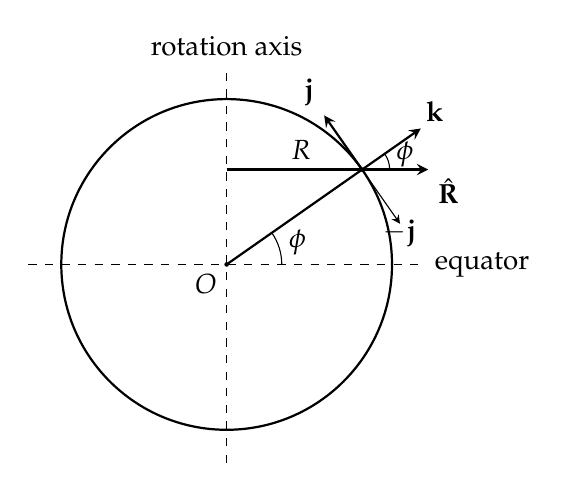
\begin{tikzpicture}[scale=0.7,>=stealth]

% Parameters
\def\a{3.0}
\def\lat{35}

% Earth cross section
\draw[thick] (0,0) circle (\a);

% Rotation axis
\draw[dashed] (0,-3.6) -- (0,3.6);
\node[above] at (0,3.6) {rotation axis};

% Equatorial plane
\draw[dashed] (-3.6,0) -- (3.6,0);
\node[right] at (3.6,0) {equator};

% Center
\coordinate (O) at (0,0);
\fill (O) circle (1.2pt);
\node[below left] at (O) {$O$};

% Surface point at latitude phi
\coordinate (P) at ({\a*cos(\lat)},{\a*sin(\lat)});
\fill (P) circle (1.2pt);

% Radius to P
\draw[thick] (O) -- (P);

% Latitude angle at center
\draw (1.0,0) arc[start angle=0,end angle=\lat,radius=1.0];
\node at ({1.35*cos(\lat/2)},{1.35*sin(\lat/2)}) {$\phi$};

% Point on rotation axis at same height as P
\coordinate (A) at (0,{ \a*sin(\lat) });

% Vector from rotation axis to P
\draw[thick] (A) -- (P);
\node[above] at ($(A)!0.55!(P)$) {$R$};

% Local basis vectors at P
\draw[->,thick] (P) -- ++({\lat}:1.3);
\node[above right] at ($(P)+({\lat}:1.2)$) {$\mathbf{k}$};

\draw[->,thick] (P) -- ++({\lat+90}:1.2);
\node[above left] at ($(P)+({\lat+90}:1.2)$) {$\mathbf{j}$};

% R-hat at P
\draw[->,thick] (P) -- ++(0:1.2);
\node[below right] at ($(P)+(1.2,0)$) {$\hat{\mathbf{R}}$};

% Angle between k and R-hat
\draw ($(P)+(0.5,0)$) arc[start angle=0,end angle=\lat,radius=0.5];
\node at ($(P)+(0.78,0.28)$) {$\phi$};

% Optional small arrow showing -j component direction
\draw[->] (P) -- ++({\lat-90}:1.2);
\node[left] at ($(P)+({\lat-80}:1.65)$) {$-\mathbf{j}$};

\end{tikzpicture}

\caption{Geometry of the unit vector $\hat{\mathbf{R}}$, directed outward from Earth's rotation axis. At latitude $\phi$, $\hat{\mathbf{R}}$ lies in the local meridional--vertical plane and can be decomposed into an equatorward horizontal component $-\sin\phi\,\mathbf{j}$ and an upward vertical component $\cos\phi\,\mathbf{k}$.}
\label{fig:c1_rhat_decomposition}
\end{figure}

Because of its zonal motion, the air parcel's total angular velocity is

\begin{equation}
    \Omega + \frac{u}{R},
\end{equation}

where $u/R$ is its angular velocity relative to Earth. The centrifugal acceleration is therefore larger than that of an object at rest relative to Earth. The excess centrifugal acceleration is

\begin{equation}
    \left(\Omega+\frac{u}{R}\right)^2R-\Omega^2R = 2\Omega u+\frac{u^2}{R},
\end{equation}

and is directed outward from the rotation axis.

The outward direction from Earth's rotation axis lies in the local meridional--vertical plane. At latitude $\phi$, this direction can be decomposed into a horizontal meridional component and a vertical component (see Fig.~\ref{fig:c1_rhat_decomposition}). Geometrically,

\begin{equation}
    \hat{\mathbf{R}} = -\sin\phi\,\mathbf{j} + \cos\phi\,\mathbf{k},
\end{equation}

where $\hat{\mathbf{R}}$ is the unit vector directed outward from Earth's rotation axis, $\mathbf{j}$ is the local northward unit vector, and $\mathbf{k}$ is the local upward unit vector. The negative sign indicates that the horizontal component points equatorward in the Northern Hemisphere, whereas the vertical component points upward. Therefore, the outward direction has a northward component $-\sin\phi$ and an upward component $\cos\phi$.

Taking $v$ as positive northward and $w$ as positive upward,

\begin{equation}
    \frac{Dv}{Dt}
    = -\left(2\Omega u+\frac{u^2}{R}\right)\sin\phi = -2\Omega u\sin\phi-\frac{u^2}{r}\tan\phi,
\label{eq:c1_meridional_acceleration}
\end{equation}

where $R=r\cos\phi$ has been used. Similarly,

\begin{equation}
    \frac{Dw}{Dt} = \left(2\Omega u+\frac{u^2}{R}\right)\cos\phi = 2\Omega u\cos\phi+\frac{u^2}{r}.
\label{eq:c1_vertical_acceleration}
\end{equation}

Again, the terms proportional to $2\Omega u$ are the meridional and vertical components of the Coriolis acceleration, and the terms proportional to $u^2/r$ are the curvature effects.

Because Earth's radius is large, the terms proportional to $1/r$ in Eqs.~\ref{eq:c1_zonal_acceleration}--\ref{eq:c1_vertical_acceleration}, which represent curvature effects, are generally negligible for large-scale atmospheric motion. In Eq.~\ref{eq:c1_zonal_acceleration}, the Coriolis term $-2\Omega w\cos\phi$ is also usually small because $w$ is small. In Eq.~\ref{eq:c1_vertical_acceleration}, the vertical Coriolis acceleration $2\Omega u\cos\phi$ is generally small compared with the dominant vertical forces, particularly gravity. With these approximations, retaining only the horizontal Coriolis terms in Eq.~\ref{eq:c1_zonal_acceleration} and Eq.~\ref{eq:c1_meridional_acceleration} gives

\begin{equation}
    \frac{D u}{D t} = 2\Omega v\sin\phi = fv, \qquad
    \frac{D v}{D t} = -2\Omega u\sin\phi = -fu,
\label{eq:c1_horizontal_coriolis}
\end{equation}

where

\begin{equation}
    f = 2\Omega\sin\phi
\end{equation}

is the \textit{Coriolis parameter}.

In the Northern Hemisphere, $f>0$ for $0\leq\phi\leq\pi/2$. An eastward-moving parcel $(u>0)$ is accelerated southward, and a northward-moving parcel $(v>0)$ is accelerated eastward. In both cases, the Coriolis acceleration is directed to the right of the motion.

In the Southern Hemisphere, $f<0$ for $-\pi/2\leq\phi\leq0$, so the signs of the Coriolis accelerations are reversed and the parcel is deflected to the left of its motion.

Consider the horizontal velocity $\mathbf{v}_h=u\mathbf{i}+v\mathbf{j}$ and the Coriolis acceleration $\mathbf{a}_C=fv\mathbf{i}-fu\mathbf{j}$. Their dot product is

\begin{equation}
    \mathbf{v}_h\cdot\mathbf{a}_C = u(fv)+v(-fu)=0.
\end{equation}

In other words, the Coriolis acceleration is perpendicular to the horizontal velocity in both hemispheres. When the Coriolis acceleration is the only horizontal acceleration, the rate of change of the squared horizontal \textit{speed} is

\begin{equation}
\begin{aligned}
    \frac{D}{Dt}|\mathbf{v}_h|^2
    &= \frac{D}{Dt}(u^2+v^2) = 2u\frac{Du}{Dt}+2v\frac{Dv}{Dt} \\
    &= 2u(fv)+2v(-fu)=0.
\end{aligned}
\end{equation}

Thus, $|\mathbf{v}_h|$ remains constant even though the velocity vector continuously changes direction. Geometrically, the Coriolis acceleration turns the velocity vector without changing its length, analogous to the centripetal acceleration in uniform circular motion. For constant $f$, its magnitude is $|\mathbf{a}_C|=|f||\mathbf{v}_h|$, which can be nonzero even when the speed is constant. Since the acceleration is perpendicular to the velocity, it does no work on the parcel and cannot change its horizontal kinetic energy. Other forces, such as the pressure gradient force, may still change the parcel's speed.

The acceleration equations derived in this section describe only the effects of Earth's rotation and spherical-coordinate curvature. They are not the complete atmospheric momentum equations. Furthermore, the simplified horizontal equations in Eq.~\ref{eq:c1_horizontal_coriolis} retain only the leading horizontal Coriolis terms, neglecting the additional zonal Coriolis term $-2\Omega w\cos\phi$ and the curvature terms $(uv\tan\phi-uw)/r$ and $-(u^2\tan\phi+vw)/r$. The vertical acceleration equation, which includes the Coriolis term $2\Omega u\cos\phi$ and the curvature term $(u^2+v^2)/r$, is also omitted. A complete treatment of the Coriolis force and the atmospheric momentum equations will be presented in Chapter~2.

\section{Structure of the Static Atmosphere}

The thermodynamic state of the atmosphere at any point is characterized by pressure, temperature, and density (or specific volume). These variables are related through the equation of state. For dry air, which can be approximated as an ideal gas,

\begin{equation}
    p\alpha=R_dT, \qquad p=\rho R_dT,
\label{eq:c1_ideal_gas_law}
\end{equation}

where $p$ is pressure, $T$ is absolute temperature, $\rho$ is density, $\alpha=\rho^{-1}$ is specific volume, and $R_d=287\ \mathrm{J\,kg^{-1}\,K^{-1}}$ is the specific gas constant for dry air. Pressure, temperature, and density are all functions of position and time, but remain constrained by Eq.~\ref{eq:c1_ideal_gas_law} locally in the atmosphere.

\subsection{The Hydrostatic Equation}

In an atmosphere at rest, the downward gravitational force must be balanced by the upward vertical pressure gradient force. This condition is known as \textit{hydrostatic balance}. To derive it, consider a thin horizontal layer of air with cross-sectional area $A$ and infinitesimal thickness $\delta z$, extending from geometric height $z$ to $z+\delta z$.

\begin{figure}[t]
\centering
\resizebox{0.6\columnwidth}{!}{%
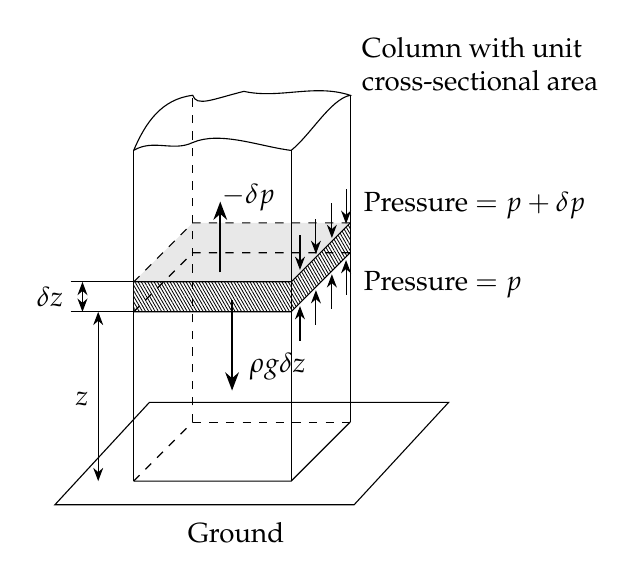
\begin{tikzpicture}[>=Stealth,scale=1]

% Ground plane
\draw
    (-1.0,-0.3) -- (2.8,-0.3) -- (4.0,1.0)
    -- (0.2,1.0) -- cycle;
\node at (1.3,-0.65) {Ground};

% Column geometry
\def\W{2.0}
\def\D{0.75}
\def\H{4.2}
\def\Z{2.15}
\def\dZ{0.38}

% Shaded atmospheric layer: upper face
\fill[gray!18]
    (0,\Z+\dZ) -- (2,\Z+\dZ)
    -- (2.75,\Z+\dZ+0.75)
    -- (0.75,\Z+\dZ+0.75) -- cycle;

% Front face
\fill[white] (0,\Z) rectangle (2,\Z+\dZ);
\draw[
    pattern={Lines[angle=120,distance=1pt,line width=0.3pt]},
    pattern color=black
] (0,\Z) rectangle (2,\Z+\dZ);

% Right face
\fill[white]
    (2,\Z) -- (2.75,\Z+0.75)
    -- (2.75,\Z+\dZ+0.75)
    -- (2,\Z+\dZ) -- cycle;
\fill[
    pattern={Lines[angle=120,distance=1pt,line width=0.3pt]},
    pattern color=black
]
    (2,\Z) -- (2.75,\Z+0.75)
    -- (2.75,\Z+\dZ+0.75)
    -- (2,\Z+\dZ) -- cycle;

% Hidden edges
\draw[dashed,thin] (0.75,0.75) -- (0.75,4.9);
\draw[dashed,thin] (0,0) -- (0.75,0.75);
\draw[dashed,thin] (0.75,0.75) -- (2.75,0.75);

% Vertical edges
\draw (0,0) -- (0,\H);
\draw (2,0) -- (2,\H);
\draw (2.75,0.75) -- (2.75,4.9);

% Bottom edges
\draw (0,0) -- (2,0) -- (2.75,0.75);

% Top irregular surface
\draw
    (0,4.2)
    .. controls (0.25,4.35) and (0.5,4.18) .. (0.75,4.3)
    .. controls (1.1,4.45) and (1.6,4.25) .. (2,4.2)
    .. controls (2.25,4.4) and (2.5,4.85) .. (2.75,4.9)
    .. controls (2.3,5.05) and (1.85,4.85) .. (1.4,4.95)
    .. controls (1.0,4.85) and (0.8,4.75) .. (0.75,4.9)
    .. controls (0.35,4.85) and (0.15,4.55) .. (0,4.2);

% Unit cross-sectional area
\node[align=left] at (4.4,5.3)
    {Column with unit\\cross-sectional area};

% Slab outlines
\draw
    (0,\Z) -- (2,\Z) -- (2.75,\Z+0.75);
\draw
    (0,\Z+\dZ) -- (2,\Z+\dZ)
    -- (2.75,\Z+\dZ+0.75);
\draw
    (2,\Z) -- (2,\Z+\dZ);
\draw
    (2.75,\Z+0.75) -- (2.75,\Z+\dZ+0.75);

% Back edges of slab
\draw[dashed,thin]
    (0,\Z) -- (0.75,\Z+0.75)
    -- (2.75,\Z+0.75);
\draw[dashed,thin]
    (0,\Z+\dZ) -- (0.75,\Z+\dZ+0.75)
    -- (2.75,\Z+\dZ+0.75);

% Downward pressure arrows on upper surface
\foreach \t in {0.15,0.42,0.69,0.93} {
    \pgfmathsetmacro{\xx}{2+0.75*\t}
    \pgfmathsetmacro{\yy}{\Z+\dZ+0.75*\t}
    \draw[->,thin]
        (\xx,\yy+0.48) -- (\xx,\yy+0.04);
}

% Upward pressure arrows on lower surface
\foreach \t in {0.15,0.42,0.69,0.93} {
    \pgfmathsetmacro{\xx}{2+0.75*\t}
    \pgfmathsetmacro{\yy}{\Z+0.75*\t}
    \draw[->,thin]
        (\xx,\yy-0.48) -- (\xx,\yy-0.04);
}

% Pressure labels
\node[right] at (2.8,3.5) {Pressure $=p+\delta p$};
\node[right] at (2.8,2.5) {Pressure $=p$};

% Net upward pressure force
\draw[->,thick] (1.1,2.65) -- (1.1,3.55);
\node[right] at (1.0,3.6) {$-\delta p$};

% Gravitational force
\draw[->,thick] (1.25,2.3) -- (1.25,1.15);
\node[right] at (1.35,1.45) {$\rho g\delta z$};

% Height z
\draw[<->,thin] (-0.45,0) -- (-0.45,\Z);
\node[left] at (-0.45,1.05) {$z$};

% Layer thickness dz
\draw[<->,thin]
    (-0.65,\Z) -- (-0.65,\Z+\dZ);
\draw[thin]
    (-0.8,\Z) -- (0,\Z);
\draw[thin]
    (-0.8,\Z+\dZ) -- (0,\Z+\dZ);
\node[left] at (-0.77,\Z+0.5*\dZ) {$\delta z$};

\end{tikzpicture}%
}
\caption{Balance of forces under hydrostatic equilibrium. A thin atmospheric layer of thickness $\delta z$ and unit horizontal cross-sectional area is subjected to upward pressure $p$ on its lower surface, downward pressure $p+\delta p$ on its upper surface, and downward gravitational force $\rho g\,\delta z$. Since $\delta p<0$, the net upward pressure force is $-\delta p$.}
\label{fig:c1_hydrostatic_balance}
\end{figure}

The pressure exerted on the lower surface produces an upward force $F_{\mathrm{bottom}}=p(z)A$, whereas the pressure on the upper surface produces a downward force $F_{\mathrm{top}}=p(z+\delta z)A$. The gravitational force acting on the air within the layer is directed downward and has magnitude $F_g=\rho gA\,\delta z$, where $\rho$ and $g$ are evaluated within the infinitesimally thin layer. Therefore, vertical force balance requires

\begin{equation}
    p(z)A-p(z+\delta z)A-\rho gA\,\delta z=0.
\end{equation}

Expanding the pressure at the upper surface using a first-order Taylor approximation,

\begin{equation}
    p(z+\delta z)=p(z) + \frac{dp}{dz}\delta z,
\end{equation}

and substituting into the force balance gives

\begin{equation}
    -\frac{dp}{dz}A\,\delta z-\rho gA\,\delta z=0.
\end{equation}

Dividing by $A\,\delta z$ yields the \textit{hydrostatic equation},

\begin{equation}
    \frac{dp}{dz}=-\rho g.
\label{eq:c1_hydrostatic}
\end{equation}

Since $\rho>0$ and $g>0$, the vertical pressure gradient is negative, indicating that atmospheric pressure decreases with increasing height. Physically, the pressure difference between the lower and upper surfaces of an air layer must support the weight of the air contained within that layer.

Although derived for an atmosphere at rest, hydrostatic balance provides an excellent approximation for the vertical pressure distribution in most large-scale atmospheric motions. This is because vertical accelerations are generally small compared with gravitational acceleration. Significant departures from hydrostatic balance can occur in intense small-scale systems, such as squall lines and tornadoes, where vertical accelerations become dynamically important.

Integrating Eq.~\ref{eq:c1_hydrostatic} from height $z$ to the top of the atmosphere, where pressure approaches zero, gives

\begin{equation}
    \int_{p(z)}^0 dp = -\int_z^\infty \rho(z)g(z)\,dz \Longrightarrow p(z) = \int_z^\infty \rho(z)g(z)\,dz.
\label{eq:c1_pressure_column}
\end{equation}

Here, $\rho(z)$ and $g(z)$ are functions of geometric height $z$. Equation~\ref{eq:c1_pressure_column} shows that atmospheric pressure at any height equals the weight per unit horizontal area of the overlying air column. Thus, mean sea level pressure, approximately $1013.25\ \mathrm{hPa}$, corresponds to the weight per unit area of the entire atmospheric column above sea level. Approximating gravity as constant $g_0 = 9.80665\ \mathrm{ms^{-2}}$, the mass of this atmospheric column over the unit area is

\begin{equation}
    \int_0^\infty \rho(z)\,dz \approx \frac{p(0)}{g_0} = \frac{101325\ \mathrm{Pa}}{9.80665\ \mathrm{ms^{-2}}} \approx 10339.3\ \mathrm{kg}.
\end{equation}

\subsection{Geopotential and Geopotential Height}

Because gravitational acceleration varies with altitude, geometric height is not always the most convenient vertical coordinate for atmospheric dynamics. A more physically meaningful quantity is the \textit{geopotential} $\Phi$, defined as the gravitational potential energy per unit mass relative to a reference level. Taking sea level as the reference,

\begin{equation}
    \Phi(z)=\int_0^z g(z)\,dz, \qquad d\Phi=g(z)\,dz,
\label{eq:c1_geopotential_static}
\end{equation}

where $\Phi$ has units of $\mathrm{m^2\,s^{-2}}$. The geopotential represents the work per unit mass required to raise an air parcel from the reference level to height $z$ against gravity.

The \textit{geopotential height} $Z$ is defined by

\begin{equation}
    Z=\frac{\Phi}{g_0} = \frac{1}{g_0}\int_0^z g(z)\,dz,
\label{eq:c1_geopotential_height_static}
\end{equation}

where $g_0=9.80665\ \mathrm{m\,s^{-2}}$ is the standard gravitational acceleration at mean sea level. Geopotential height has units of length and represents the height that would produce the same geopotential in a uniform gravitational field of strength $g_0$.

To examine the relationship between geometric height and geopotential height, consider an idealized spherical Earth with radius $a\approx6371\ \mathrm{km}$. Neglecting variations due to Earth's rotation and nonspherical mass distribution, gravitational acceleration at distance $r=a+z$ from Earth's center is

\begin{equation}
    g(z)\approx\frac{GM}{(a+z)^2} = \frac{GM}{a^2}\frac{a^2}{(a+z)^2} = g_0\left(\frac{a}{a+z}\right)^2,
\end{equation}

where $G$ is the universal gravitational constant and $M$ is Earth's mass. Here, $g_0 = GM/a^2$ is assumed for this idealized model. Substituting into Eq.~\ref{eq:c1_geopotential_height_static},

\begin{equation}
\begin{aligned}
    Z(z)
    &=\frac{1}{g_0}\int_0^z g_0\left(\frac{a}{a+z}\right)^2 dz\\
    &=a^2\left[-\frac{1}{a+z}\right]_0^z
    =\frac{az}{a+z}.
\end{aligned}
\label{eq:c1_geopotential_geometric_relation}
\end{equation}

For atmospheric heights much smaller than Earth's radius, $z\ll a$, we obtain $Z\approx z$. However, because gravitational acceleration decreases with altitude, geopotential height is always slightly smaller than geometric height in this idealized model. Their difference is

\begin{equation}
    z-Z=z-\frac{az}{a+z}=\frac{z^2}{a+z}.
\end{equation}

For example, the differences are approximately $16\ \mathrm{m}$ at $z=10\ \mathrm{km}$, $390\ \mathrm{m}$ at $z=50\ \mathrm{km}$, and $1.5\ \mathrm{km}$ at $z=100\ \mathrm{km}$. Thus, geometric and geopotential heights are nearly identical in the troposphere and lower stratosphere, but their difference becomes increasingly important at higher altitudes.

\subsection{The Hypsometric Equation}

The hydrostatic equation can be expressed in terms of geopotential rather than geometric height. Combining Eq.~\ref{eq:c1_hydrostatic} with $d\Phi=g\,dz$ gives

\begin{equation}
    dp=-\rho g\,dz=-\rho\,d\Phi.
\end{equation}

Rearranging and using the specific volume $\alpha=\rho^{-1}$,

\begin{equation}
    d\Phi=-\alpha\,dp.
\end{equation}

From the ideal gas equation, $\alpha=R_dT/p$. Therefore,

\begin{equation}
    d\Phi=-\frac{R_dT}{p}dp=-R_dT\,d\ln p.
\label{eq:c1_hydrostatic_geopotential}
\end{equation}

This expression shows that the variation of geopotential with logarithmic pressure depends directly on temperature. Integrating between two pressure surfaces $p_1$ and $p_2$, with $p_1>p_2$ and corresponding geopotential heights $Z_1$ and $Z_2$, gives

\begin{equation}
    \Phi_2-\Phi_1 = -R_d\int_{p_1}^{p_2}T\,d\ln p = R_d\int_{p_2}^{p_1}T\,d\ln p.
\end{equation}

Since $\Phi=g_0Z$, we obtain the \textit{hypsometric equation},

\begin{equation}
    Z_2-Z_1=\frac{R_d}{g_0}\int_{p_2}^{p_1}T\,d\ln p.
    \label{eq:c1_hypsometric}
\end{equation}

The temperature $T$ in this integral is evaluated along the vertical atmospheric column and may vary with pressure. Eq.~\ref{eq:c1_hypsometric} indicates that layer thickness depends on the vertical temperature distribution.

To simplify the expression, define the layer-mean temperature weighted by logarithmic pressure,

\begin{equation}
    \langle T\rangle = \left[\int_{p_2}^{p_1}d\ln p\right]^{-1} \int_{p_2}^{p_1}T\,d\ln p.
\end{equation}

Since

\begin{equation}
    \int_{p_2}^{p_1}d\ln p=\ln\left(\frac{p_1}{p_2}\right),
\end{equation}

the hypsometric equation becomes

\begin{equation}
    \Delta T = Z_2 - Z_1 = \frac{R_d\langle T\rangle}{g_0} \ln\left(\frac{p_1}{p_2}\right).
\label{eq:c1_hypsometric_mean_temperature}
\end{equation}

Introducing the layer-mean \textit{scale height}

\begin{equation}
    H=\frac{R_d\langle T\rangle}{g_0},
\end{equation}

which has units of length (m), we obtain

\begin{equation}
    \Delta Z=H\ln\left(\frac{p_1}{p_2}\right).
\label{eq:c1_layer_thickness}
\end{equation}

The hypsometric equation shows that the thickness between two fixed pressure surfaces depends solely on the layer-mean temperature, to which it is directly proportional. A warmer atmospheric layer has a greater thickness because warmer air is less dense at a given pressure, causing pressure to decrease more slowly with height. Conversely, a colder layer is thinner because pressure decreases more rapidly with height.

One direct implication of the hypsometric equation is that geopotential thickness and layer-mean temperature have identical horizontal spatial patterns between two fixed pressure surfaces. When mean sea level is chosen as the reference surface ($Z_1=0$), the geopotential height of a pressure surface depends on both the mean temperature of the underlying atmospheric layer and the horizontally varying sea-level pressure. Consequently, the horizontal pattern of geopotential height does not necessarily coincide with that of temperature at the same pressure level.

\subsection{The Isothermal Atmosphere}

Under the assumption of an \textit{isothermal atmosphere}, in which temperature is constant with height, the scale height is also constant,

\begin{equation}
    H=\frac{R_dT}{g_0}.
\end{equation}

Taking $Z_1=0$, $p_1=p_0$, $Z_2=Z$, and $p_2=p$ in Eq.~\ref{eq:c1_layer_thickness} yields

\begin{equation}
    Z=H\ln\left(\frac{p_0}{p}\right),
\end{equation}

where $p_0$ is the pressure at the reference geopotential height $Z=0$. Rearranging gives

\begin{equation}
    p(Z)=p_0e^{-Z/H}.
    \label{eq:c1_isothermal_pressure}
\end{equation}

Thus, atmospheric pressure decreases exponentially with geopotential height in an isothermal atmosphere. At $Z=H$, pressure is reduced to $p_0/e$, approximately $36.8\%$ of its reference value. Each additional scale height reduces the pressure by another factor of $e^{-1}$.

\subsection{Pressure as a Vertical Coordinate}

The hydrostatic equation establishes a monotonic relationship between pressure and geometric height within each atmospheric column. Since $dp/dz=-\rho g<0$, pressure decreases continuously with increasing height, allowing pressure to be used as an alternative vertical coordinate.

In geometric-height coordinates, atmospheric variables may be expressed as functions of $(x,y,z,t)$, where $x$ and $y$ denote the eastward and northward horizontal coordinates, respectively, and $z$ is geometric height. When pressure is used as the vertical coordinate, geometric height becomes a dependent variable, and the atmospheric state can instead be described by fields such as

\begin{equation}
    \Phi=\Phi(x,y,p,t), \qquad T=T(x,y,p,t).
\end{equation}

A surface of constant pressure is called an \textit{isobaric surface}. Unlike a surface of constant geometric height, an isobaric surface generally varies in elevation.

One important consequence of using pressure coordinates is that the horizontal pressure gradient force can be expressed in terms of the horizontal gradient of geopotential evaluated at constant pressure. To demonstrate this transformation, consider the horizontal $x$ direction in the $(x,z)$ plane.

Since pressure depends on both horizontal position and geometric height, $p=p(x,z)$, a small horizontal displacement $\delta x$ at constant height produces a pressure change

\begin{equation}
    \delta p_x \approx \left(\frac{\partial p}{\partial x}\right)_z\delta x,
\end{equation}

where the subscript $z$ indicates that geometric height is held constant during differentiation. $(\partial p/\partial x)_z$ represents the horizontal pressure gradient along a surface of constant geometric height. Similarly, a small vertical displacement $\delta z$ at constant horizontal position produces a pressure change

\begin{equation}
    \delta p_z \approx \left(\frac{\partial p}{\partial z}\right)_x\delta z,
\end{equation}

Along an isobaric surface, the total pressure change must vanish. Therefore, these two pressure changes cancel,

\begin{equation}
    \delta p_x+\delta p_z\approx
    \left(\frac{\partial p}{\partial x}\right)_z\delta x + \left(\frac{\partial p}{\partial z}\right)_x\delta z=0.
\end{equation}

Rearranging and dividing by $\delta x$ gives, to first order,

\begin{equation}
    \left(\frac{\partial p}{\partial x}\right)_z \approx-\left(\frac{\partial p}{\partial z}\right)_x \frac{\delta z}{\delta x}.
\end{equation}

Taking the limit as $\delta x\to0$ along the isobaric surface gives

\begin{equation}
\begin{aligned}
    \left(\frac{\partial p}{\partial x}\right)_z
    &= -\left(\frac{\partial p}{\partial z}\right)_x
    \lim_{\delta x\to0}\left(\frac{\delta z}{\delta x}\right)_p\\
    &= -\left(\frac{\partial p}{\partial z}\right)_x \left(\frac{\partial z}{\partial x}\right)_p.
\end{aligned}
\label{eq:c1_pressure_gradient_transform}
\end{equation}

Here, the subscript $p$ indicates that pressure is held constant, so $(\partial z/\partial x)_p$ represents the slope of an isobaric surface. Substituting the hydrostatic relation $(\partial p/\partial z)_x=-\rho g$ into Eq.~\ref{eq:c1_pressure_gradient_transform} yields

\begin{equation}
    \left(\frac{\partial p}{\partial x}\right)_z
    =\rho g\left(\frac{\partial z}{\partial x}\right)_p.
\end{equation}

Therefore, the horizontal pressure gradient force per unit mass in the $x$ direction becomes

\begin{equation}
    -\frac{1}{\rho}\left(\frac{\partial p}{\partial x}\right)_z
    =-g\left(\frac{\partial z}{\partial x}\right)_p
    =-\left(\frac{\partial\Phi}{\partial x}\right)_p.
\label{eq:c1_pgf_pressure_x}
\end{equation}

Similarly, for the $y$ direction,

\begin{equation}
    -\frac{1}{\rho}\left(\frac{\partial p}{\partial y}\right)_z
    =-\left(\frac{\partial\Phi}{\partial y}\right)_p.
\label{eq:c1_pgf_pressure_y}
\end{equation}

Combining the two horizontal directions, the pressure gradient force per unit mass in isobaric coordinates can be written as

\begin{equation}
\begin{aligned}
    \frac{\mathbf{F}_{p,h}}{m}
    &=-\frac{1}{\rho}\left(\frac{\partial p}{\partial x}\right)_z\mathbf{i} - \frac{1}{\rho}\left(\frac{\partial p}{\partial y}\right)_z\mathbf{j}\\
    &=-\left(\frac{\partial\Phi}{\partial x}\right)_p\mathbf{i}
    -\left(\frac{\partial\Phi}{\partial y}\right)_p\mathbf{j}
    =-\nabla_p\Phi,
\label{eq:c1_pgf_isobaric}
\end{aligned}
\end{equation}

where $\nabla_p$ denotes the horizontal gradient operator evaluated along a constant-pressure surface.

Thus, in pressure coordinates, the horizontal pressure gradient force can be determined from the gradient of geopotential along an isobaric surface. The density $\rho$ no longer appears explicitly in the expression, which is a major advantage of pressure coordinates in atmospheric dynamics.

Pressure coordinates also provide a useful physical intuition. A constant-pressure surface may have different geopotential heights due to horizontal temperature variations, as described by the hypsometric equation. The pressure gradient force accelerates air from higher to lower geopotential along this surface, much like water flowing downhill under gravity, thereby linking the thermal structure of the atmosphere to horizontal pressure gradients and atmospheric circulation.

\subsection{A Generalized Vertical Coordinate}

Any single-valued, monotonic function of pressure or height can be used as an independent vertical coordinate. For example, many numerical weather prediction models employ the \textit{sigma coordinate}, defined as

\begin{equation}
    \sigma=\frac{p(x,y,z,t)}{p_s(x,y,t)},
\end{equation}

where $p_s$ is the atmospheric pressure at the ground. At the surface, $p=p_s$, so $\sigma=1$ regardless of variations in surface pressure. Consequently, the ground always coincides with a constant-coordinate surface, making sigma coordinates particularly useful in regions with complex topography.

More generally, consider a vertical coordinate $s=s(x,y,z,t)$ that is a single-valued, monotonic function of geometric height $z$. The coordinate $s$ need not represent pressure or height directly, but its monotonicity ensures a unique correspondence with height, allowing the coordinate transformation to be inverted.

\subsection{A Generalized Vertical Coordinate}

The pressure-coordinate system introduced in the previous section is a special case of a more general approach in which any single-valued, monotonic function of pressure or height can serve as the independent vertical coordinate. For example, many numerical weather prediction models use the \textit{sigma coordinate}, defined as

\begin{equation}
    \sigma=\frac{p(x,y,z,t)}{p_s(x,y,t)},
\end{equation}

where $p_s$ is the atmospheric pressure at the ground. Since $p=p_s$ at the surface, $\sigma=1$ regardless of variations in surface pressure. Thus, the ground always coincides with a constant-coordinate surface, making sigma coordinates particularly useful in regions with complex topography.

More generally, consider a vertical coordinate $s=s(x,y,z,t)$ that is a single-valued, monotonic function of geometric height $z$. The coordinate $s$ need not represent pressure or height directly, but its monotonicity ensures a unique correspondence with height, allowing the coordinate transformation to be inverted.

In the previous section, the horizontal pressure gradient was transformed by considering displacements along an isobaric surface, where the total pressure change vanishes. The same approach can be extended to a surface of constant $s$, with one important difference: pressure is generally not constant along this surface,

\begin{equation}
    \delta p_s = \delta p_x+\delta p_z \approx\left(\frac{\partial p}{\partial x}\right)_z\delta x + \left(\frac{\partial p}{\partial z}\right)_x\delta z \ne 0.
\end{equation}

Dividing by $\delta x$ and taking the limit as $\delta x\to0$ along the constant-$s$ surface gives

\begin{equation}
\begin{aligned}
    \left(\frac{\partial p}{\partial x}\right)_s
    &=\left(\frac{\partial p}{\partial x}\right)_z
    +\left(\frac{\partial p}{\partial z}\right)_x
    \lim_{\delta x\to0}\left(\frac{\delta z}{\delta x}\right)_s\\
    &=\left(\frac{\partial p}{\partial x}\right)_z
    +\left(\frac{\partial p}{\partial z}\right)_x
    \left(\frac{\partial z}{\partial x}\right)_s.
\end{aligned}
\label{eq:c1_general_pressure_transform}
\end{equation}

Here, the $(\partial z/\partial x)_s$ represents the slope of a constant-$s$ surface. Rearranging Eq.~\ref{eq:c1_general_pressure_transform} and multiplying by $-1/\rho$ gives the horizontal pressure gradient force per unit mass,

\begin{equation}
    -\frac{1}{\rho}\left(\frac{\partial p}{\partial x}\right)_z = -\frac{1}{\rho}\left(\frac{\partial p}{\partial x}\right)_s + \frac{1}{\rho}\left(\frac{\partial p}{\partial z}\right)_x \left(\frac{\partial z}{\partial x}\right)_s.
\end{equation}

Under hydrostatic balance, $(\partial p/\partial z)_x=-\rho g$, so

\begin{equation}
    -\frac{1}{\rho}\left(\frac{\partial p}{\partial x}\right)_z = -\frac{1}{\rho}\left(\frac{\partial p}{\partial x}\right)_s - g\left(\frac{\partial z}{\partial x}\right)_s.
\label{eq:c1_general_pgf_hydrostatic_x}
\end{equation}

The first term on the right represents the pressure variation along a constant-$s$ surface, and the second accounts for the slope of that surface in the gravitational field. Applying the same transformation in the $y$ direction gives

\begin{equation}
    -\frac{1}{\rho}\left(\frac{\partial p}{\partial y}\right)_z = -\frac{1}{\rho}\left(\frac{\partial p}{\partial y}\right)_s - g\left(\frac{\partial z}{\partial y}\right)_s.
\label{eq:c1_general_pgf_hydrostatic_y}
\end{equation}

The connection with the previous section becomes clear by choosing $s=p$. In this special case, Eqs.~\ref{eq:c1_general_pgf_hydrostatic_x} and \ref{eq:c1_general_pgf_hydrostatic_y} reduce to Eqs.~\ref{eq:c1_pgf_pressure_x} and \ref{eq:c1_pgf_pressure_y}, respectively. In later chapters, we will apply these generalized transformations to express the dynamical equations in different vertical coordinate systems.



\end{document}
